\documentclass[hyperref=unicode,graphics=pdflatex,12pt]{beamer}

\usepackage[T2A]{fontenc}
\usepackage[utf8]{inputenc}
\usepackage[russian]{babel}


\mode<presentation>
{
  \setbeamercovered{invisible}
}

\usepackage{amssymb,amsthm,amsmath,amsfonts,array,pstcol,graphicx,pst-node,comment,rotating,ccaption,beamerthemesplit}

\def\sgn{\text{sgn}\,}

\useoutertheme{infolines}
\setbeamertemplate{theorems}[numbered]
\setbeamertemplate{footline}[page number]{}
\setbeamertemplate{headline}{}

\deftranslation{Theorem}{Теорема}
\deftranslation{Lemma}{Лемма}
\deftranslation{Definition}{Определение}

\begin{document}

\title{Поиск Абелевых строк наибольшей длины}
\author{И.~Збань\\
Научный руководитель: В.~Аксёнов}

\date{\today}
\institute{
\includegraphics[width=0.3\textwidth]{pics/itmo.png}}
\frame{\titlepage}                                   

\begin{comment}
\begin{frame}{}
  \tableofcontents
\end{frame}
\end{comment}

\section{Введение}

\begin{frame}{Постановка задачи}
Задача: Нахождение наибольшей общей Абелевой подстроки (НОАП) и поиск Абелевых подквадратов.

\vspace{0.5cm}
\onslide<2->
\begin{definition}
Две строки Абелево эквививалентны, если одна строка получается из другой перестановкой символов.
\end{definition}

\onslide<3->
\begin{definition}
Абелев подквадрат~--- подстрока, представимая как конкатенация двух Абелево эквивалентных строк.
\end{definition}
\end{frame}


\begin{frame}{Мотивация}
\hspace{0.5cm}
\begin{itemize}
\item<1-> Быстроразвивающаяся область, много публикаций за последнее время
\item<2-> Встречается как: подзадача в бионформатике (gene clusters, mass indexing),
  фильтр в задаче поиска образца с ошибками
\item<3-> Связь с известной задачей 3SUM
\end{itemize}
\end{frame}

\begin{frame}{Содержание работы}
\hspace{0.5cm}
В работе выполнены следующие части:
\begin{itemize}
\item<1-> Реализация и оценка эффективности теоретического алгоритма для решения 3SUM+
  для монотонных множеств на примере задачи о числе Абелевых подквадратов
\item<2-> Анализ задачи НОАП для бинарного алфавита
\item<3-> Решение задачи НОАП для произвольного алфавита
\end{itemize}
\end{frame}

\begin{frame}{Подсчёт числа Абелевых подквадратов}
Задача о числе Абелевых подквадратов сводится к $3SUM^+$ ($A + B = C$)
\vspace{0.5cm}

% TODO: аккуратнее описать про A, B и C
\onslide<2-> $A = B = \{(c_a(i), c_b(i))\}$, $C = \{2 \cdot c_a(i), 2 \cdot c_b(i)\}$
\vspace{0.5cm}

где $c_a(i), c_b(i)$~--- число букв $a$ и $b$ на префиксе длины $i$
\vspace{0.5cm}

\onslide<3-> и число подстрок~--- $(\#3\text{SUM}^+(A, B, C) - (n + 1)) / 2$

\end{frame}

\begin{frame}{Сравнение алгоритмов на простой строке}
Картиночка на которой видно, что квадрат работает быстро, а 1.86~--- медленно
\end{frame}

\begin{frame}{Сравнение алгоритмов на случайном тесте}
Картиночка, на которой видно, что квадрат работает быстро, а 1.86~--- оооочень медленно
\end{frame}

\begin{frame}{НОАП на бинарном алфавите}
График зависимости НОАП двух случайных бинарных строк от $n$, длины строк. Сгенерирован путем усреднения результата за $10^4$ испытаний.
\begin{center}
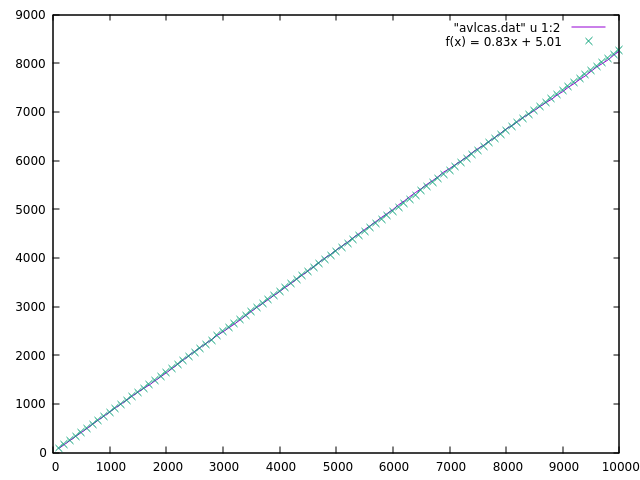
\includegraphics[width=6cm]{pics/avlcas.png}
\end{center}
\end{frame}

\begin{frame}{НОАП на бинарном алфавите}
% TODO: оценка снизу с константой
В работе доказана оценка сверху, что матождание длины НОАП двух случайных бинарных строк
ограничена сверху линейной функцией с коэффициентом меньше единицы.

Тем самым опровергнуто гипотеза из первоисточника

\vspace{0.5cm}
В работе предлагается сведение задачи к 3SUM, лучшее решение которой на данный момент имеет
асимптотику $\mathcal{O}(n^{1.86})$.
\end{frame}

\begin{frame}{НОАП на произвольном алфавите}
% TODO: Перенеси это в идею. Используя персистентные деревья с limited node copying предложен
\hspace{0.5cm}
Был разработан алгоритм решения НОАП на произвольном алфавите
за $\mathcal{O}(n^2 \log \sigma)$ времени и $\mathcal{O}(n)$ памяти.

\vspace{0.5cm}

Сравнение алгоритмов решения НОАП

\begin{center}
\begin{tabular}{|c|c|c|c|}
\hline
Год & Авторы & Время & Память \\
% это только постановка задачи
%\hline
%2013 & StringMasters & - & - \\
\hline
2015 & Кто-то & $\mathcal{O}(n^2 \sigma)$ & $\mathcal{O}(n \sigma)$ \\
\hline
2016 & Кто-то & $\mathcal{O}(n^2 \sigma)$ & $\mathcal{O}(n)$ \\
\hline
2016 & SPIRE & $\mathcal{O}(n^2 \log^2 n \log^* n)$ & $\mathcal{O}(n \log^2 n)$ \\
\hline
2017 & Я & $\mathcal{O}(n^2 \log \sigma)$ & $\mathcal{O}(n)$ \\
\hline
\end{tabular}
\end{center}
\end{frame}
      
\begin{frame}{Краткое описание алгоритма}
\vspace{0.5cm}
% TODO: Хорошо бы это разбить на пункты
\hspace{0.5cm}
Идея~--- построить персистентный массив вектора Парея для строки-конкатенации обеих данных строк,
посчитать некий хеш от каждого корня, и проверить, были ли одинаковые версии, соответствующие обеим строкам
\end{frame}

\begin{frame}{Схема вычисления хеша}
Тут какая-то непонятная картинка
\end{frame}

\begin{frame}{Вопросы?}
\begin{center}
Спасибо за внимание.
\end{center}
\end{frame}
\end{document}